% This is samplepaper.tex, a sample chapter demonstrating the
% LLNCS macro package for Springer Computer Science proceedings;
% Version 2.20 of 2017/10/04
%
\documentclass[runningheads]{llncs}
%
\usepackage{tikz}
\usetikzlibrary{arrows,shapes,positioning,shadows,trees}
\tikzset{
  basic/.style  = {draw, text width=2cm, drop shadow, font=\sffamily, rectangle},
  root/.style   = {basic, rounded corners=2pt, thin, align=center,
                   fill=green!30},
  level 2/.style = {basic, rounded corners=6pt, thin,align=center, fill=green!60,
                   text width=8em},
  level 3/.style = {basic, thin, align=left, fill=pink!60, text width=6.5em}
}

\usepackage{hyperref}
\usepackage{graphicx}
\graphicspath{{img/}}
\usepackage{tabularx}
\newcommand{\tableheadline}[1]{\multicolumn{1}{c}{#1}}
\usepackage{dirtree}
\usepackage{rotating}
\usepackage{caption}
\usepackage{booktabs}
% More space between rows:		
\renewcommand{\arraystretch}{1.1}		
% Slightly more space between columns:		
\setlength{\tabcolsep}{8pt}
\usepackage{minted}
\definecolor{dhscodebg}{rgb}{0.95,0.95,0.95} % listing background


\usepackage{xspace}
\renewcommand\UrlFont{\color{blue}\rmfamily}

\newcommand{\mypddl}{\textsc{myPddl}\xspace}
\newcommand{\mypddlclojure}{\textsc{myPddl-clojure}\xspace}
\newcommand{\mypddlsyntax}{\textsc{myPddl-syntax}\xspace}
\newcommand{\mypddldiagram}{\textsc{myPddl-diagram}\xspace}
\newcommand{\mypddlnew}{\textsc{myPddl-new}\xspace}
\newcommand{\mypddlide}{\textsc{myPddl-ide}\xspace}
\newcommand{\mypddlsnippet}{\textsc{myPddl-snippet}\xspace}
\newcommand{\mypddldistance}{\textsc{myPddl-distance}\xspace}
\newcommand{\mypddlplan}{\textsc{myPddl-plan}\xspace}
\newcommand{\pddlstudio}{\textsc{pddl studio}\xspace}
\newcommand{\itsimple}{\textsc{itSimple}\xspace}
\newcommand{\pddlmode}{\textsc{pddl}-mode\xspace}
\newcommand{\pddl}{\textsc{pddl}\xspace}
\newcommand{\uml}{\textsc{uml}\xspace}
\newcommand{\ide}{\textsc{ide}\xspace}
\newcommand{\sublimetext}{Sublime Text\xspace}


\begin{document}
%
\title{MyPDDL: Tools for efficiently creating PDDL domains and
  problems}
%
%\titlerunning{Abbreviated paper title}
% If the paper title is too long for the running head, you can set
% an abbreviated paper title here
%
\author{Volker Strobel\inst{1}\orcidID{0000-0003-2974-9827} \and
Alexandra Kirsch\inst{2}\orcidID{0000−0002−5663−1798}}
%
\authorrunning{V. Strobel and A. Kirsch}
% First names are abbreviated in the running head.
% If there are more than two authors, 'et al.' is used.
%
\institute{IRIDIA, Universit\'e Libre de Bruxelles, Belgium \and
Independent Scientist\\
\email{vstrobel@ulb.ac.be}}
%
\maketitle              % typeset the header of the contribution
%
\begin{abstract}
  The Planning Domain Definition Language (PDDL) is the
  state-of-the-art language for specifying planning problems in
  artificial intelligence research. Writing and maintaining these
  planning problems, however, can be time-consuming and error
  prone. To address this issue, we present myPDDL---a modular toolkit
  for developing and manipulating PDDL domains and problems. To
  evaluate myPDDL, we compare its features to existing knowledge
  engineering tools for PDDL. In a user test, we additionally assess
  two of its modules, namely the syntax highlighting feature and the
  type diagram generator. The users of syntax highlighting detected
  36\,\% more errors than non-users in an erroneous domain file. The
  average time on task for questions on a PDDL type hierarchy was
  reduced by 48\,\% when making the type diagram generator
  available. This implies that myPDDL can support knowledge engineers
  well in the PDDL design and analysis process.
  
\keywords{PDDL \and Planning}
\end{abstract}
%
%

\section{Introduction}
\label{sec:introduction}

Being a key aspect of artificial intelligence, \emph{planning} is
concerned with devising a sequence of actions to achieve a desired
goal \cite{helmert2008understanding}. It can be both a tool to create
automated systems and a means to support and understand human behavior
\cite{konar1999artificial}. However, the effectiveness of planning
largely depends on the quality of the problem formalization
\cite{shah2013knowledge,keps2014}. To ensure a standardized modeling
format, the Planning Domain Definition Language (\textsc{pddl})
\cite{mcdermott1998pddl} was developed and has become the de facto
standard for the description of planning tasks
\cite{ilghami2005extension}. The discipline that deals with the
integration of world information into a computer system via a human
expert is called knowledge engineering \cite{feigenbaum1983fifth}.
While automated planning could save vast amounts of time if everything
works as intended, creating the planning task specifications is a
complex task that can be error-prone and cumbersome.

The specification of Artificial Intelligence (AI) planning can be
time-consuming and cubersome. While there is a large spectrum of
different AI languages, the de facto standard language is PDDL
(\emph{Planning Domain Definition Language}). However, so far its use
is predominantly confined to academic labs. One of the reasons seems
to be the missing support of knowledge engieering tools so simplify
the task of specifying complex planning domains. 

In this chapter, we describe \mypddl
(Figure~\ref{fig:mypddl-overview}), a knowledge engineering toolkit
that supports the AI knowledge engineer in the development of complex
AI planning problems. \mypddl is intended to support knowledge
engineers throughout the entire design cycle of specifying planning
tasks. In the initial stages, it allows for the creation of structured
\textsc{pddl} projects that should encourage a disciplined design
process. With the help of snippets, i.e. code templates, often used
constructs can be inserted in \textsc{pddl} files. A syntax
highlighting feature that speeds up the error-detection can come in
handy in intermediate stages. Understanding the textual representation
of complex type hierarchies in domain files can be confusing, so an
additional tool enables their visualization. \textsc{pddl}'s limited
modeling capabilities were bypassed by developing an interface that
converts \pddl code into Clojure \cite{hickey2008clojure} code and
vice versa.  Within this project, the interface was employed for a
feature that calculates distances between objects specified in a
problem model, but the interface provides numerous other possibilities
and could also be used to further automate the modeling process. All
of the features were integrated into the customizable and extensible
Sublime Text \cite{sublimetext3} editor. Since the main aim in the
development of the toolkit was for it to be easy to use and maintain,
it is evaluated with regard to these criteria. The usability was
assessed by means of a user test with eight subjects that had no prior
experience with artificial intelligence planning. The results indicate
that both error-detection and the understanding of a given domain can
be facilitated by \mypddl.

\begin{figure}[h]
  \centering
  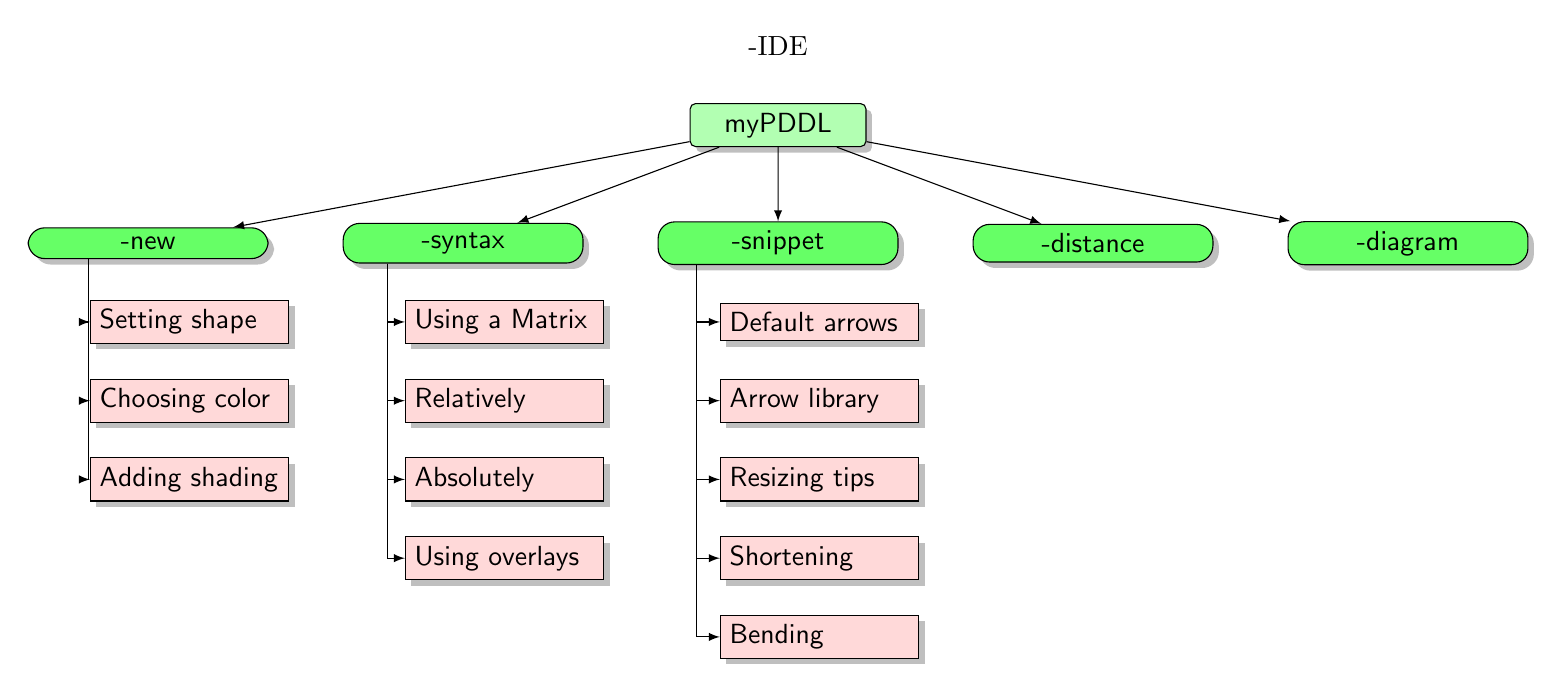
\begin{tikzpicture}[
  level 1/.style={sibling distance=40mm},
  edge from parent/.style={->,draw},
  >=latex]

  % root of the the initial tree, level 1
  \node[] (ide) {-IDE};
\node[below of = ide,root] {myPDDL}
% The first level, as children of the initial tree
  child {node[level 2] (c1) {-new}}
  child {node[level 2] (c2) {-syntax}}
  child {node[level 2] (c3) {-snippet}}
  child {node[level 2] (c4) {-distance}}
  child {node[level 2] (c5) {-diagram}};

% The second level, relatively positioned nodes
\begin{scope}[every node/.style={level 3}]
\node [below of = c1, xshift=15pt] (c11) {Setting shape};
\node [below of = c11] (c12) {Choosing color};
\node [below of = c12] (c13) {Adding shading};

\node [below of = c2, xshift=15pt] (c21) {Using a Matrix};
\node [below of = c21] (c22) {Relatively};
\node [below of = c22] (c23) {Absolutely};
\node [below of = c23] (c24) {Using overlays};

\node [below of = c3, xshift=15pt] (c31) {Default arrows};
\node [below of = c31] (c32) {Arrow library};
\node [below of = c32] (c33) {Resizing tips};
\node [below of = c33] (c34) {Shortening};
\node [below of = c34] (c35) {Bending};
\end{scope}

% lines from each level 1 node to every one of its "children"
\foreach \value in {1,2,3}
  \draw[->] (c1.195) |- (c1\value.west);

\foreach \value in {1,...,4}
  \draw[->] (c2.195) |- (c2\value.west);

\foreach \value in {1,...,5}
  \draw[->] (c3.195) |- (c3\value.west);
\end{tikzpicture}
  \caption{\mypddl is a highly customizable and extensible modular
    system, designed for supporting knowledge engineers in the process
    of writing, analyzing and expanding PDDL files and thereby
    promoting the collaboration between knowledge engineers and the
    use of PDDL in real-world applications. It consists of the parts
    shown in the figure.}
  \label{fig:mypddl-overview}
\end{figure}

The remainder of this chapter is structured as
follows. Section~\ref{sec:related-work} compares other PDDL editors
and \pddl knowledge engineering tools. Section~\ref{sec:myPDDL}
describes the different modules of \mypddl and their design
principles. Section~\ref{sec:valid-eval} compares \mypddl to the other
existing tools using a benchmark
validation. Section~\ref{sec:conclusion} concludes the chapter and
outlines future work.

\section{Related Work}
\label{sec:related-work}

This section introduces knowledge engineering tools that allow editing
\textsc{pddl} files in a textual environment. After introducing the
tools, they are compared and their shortcomings are discussed to set
the stage for \mypddl.

\pddlstudio \cite{plch2012inspect} is an application for creating and
managing \pddl projects, i.e. a collection of \pddl
files. \pddlstudio 's integrated development environment (\ide) was
inspired by Microsoft Visual Studio and imperative programming
paradigms. Its main features are syntax highlighting, error detection,
context sensitive code completion, code folding, project management,
and planner integration. \pddlstudio 's error detection can recognize
both syntactic (missing keywords, parentheses, etc.) and semantic
(wrong type of predicate parameters, misspelled predicates, etc.)
errors.

A major drawback of \pddlstudio is that it is not updated regularly
and only supports \pddl 1.2. Later \pddl versions contain several
additional features such as durative actions, numeric fluents, and
plan metrics \cite{edelkamp2004pddl2}.

\itsimple \cite{vaquero2005itsimple} follows a graphical approach
using Unified Modeling Language (\uml) diagrams. In the process
leading up to \itsimple, \textsc{uml.p} (\uml in a Planning Approach)
was proposed, a \uml variant specifically designed for modeling
planning domains and problems \cite{vaquero2006use}.

\itsimple's modeling workflow is unidirectional as changes in the
\pddl domain do not affect the \uml model and \uml models have to be
modeled manually, meaning that they cannot by generated from
\pddl. However, \cite{tonidandel2006reading} present a translation
process from a \pddl domain specification to an object-oriented
\textsc{uml.p} model as a possible integration for \itsimple. This
translation process makes extensive semantic assumptions for \pddl
descriptions. For example, the first parameter in the
\texttt{:parameters} section of an action is automatically declared as
a subclass of the default class \texttt{Agent}, and the method is
limited to predicates with a maximum arity of two. The current
version of \itsimple does not include the translation process from
\pddl to \uml.

Starting in version 4.0, \itsimple expanded its features to allow the
creation of \pddl projects from scratch (i.e. without the \uml to
\pddl translation process) \cite{vaquero2012itsimple4}. Thus far, the
\pddl editing features are basic. A minimal syntax highlighting
feature recognizes \pddl keywords, variables, and comments. \itsimple
also provides templates for \pddl constructs, such as requirement
specifications, predicates, actions, initial state, and goal
definitions.

Both \pddlstudio and \itsimple do not build on existing editors and
therefore cannot fall back on refined implementations of features that
have been modified and improved many times throughout their existence.

\pddlmode\footnote{http://rakaposhi.eas.asu.edu/planning-
  list-mailarchive/msg00085.html } for the widely used Emacs editor
builds on the sophisticated features of Emacs and uses its
extensibility and customizability. It provides syntax highlighting by
way of basic pattern matching of keywords, variables, and
comments. Additional features are automatic indentation and code
completion as well as bracket matching. Code snippets for the creation
of domains, problems, and actions are also available. Finally,
\textsc{pddl}-mode keeps track of action and problem declarations by
adding them to a menu and thus intending to allow for easy and fast
code navigation.

\pddlmode for Emacs supports \textsc{pddl} versions up to
2.2, which includes derived predicates and timed initial predicates
\cite{edelkamp2004pddl2}, but does not recognize later features like
object-fluents.

The tool editor.planning.domains allows for editing \textsc{pddl}
files online. Its feature comprise syntax highlighting, code folding,
\textsc{pddl}-specific auto-completion, and multi-tab support. The
editor is part of the Planning.Domains initiative which aims at
providing three pillars to the planning community: (1) an API for
existing planning problems; (2) a planner-in-the-cloud service; and
(3) an online PDDL editor. In contrast to \mypddl,
editor.planning.domains does not support context-aware syntax
highlighting: for example, editor.planning.domains highlights key
words even if they are misplaced. In contrast, \mypddl is aware of the
scope of a construct and highlights key words accordingly.

The tool
vscode-pddl\footnote{\url{https://marketplace.visualstudio.com/items?itemName=jan-dolejsi.pddl}}
offers a wide range of editing functions, such as syntax highlighting,
code completion, and code snippets. Since it is implemented as a
plugin for the editor Visual Studio Code, it can fall back on the the
extensibility and maturity of this code editor. In contrast to
\mypddl, it does not offer domain visualization nor an interface with
a programming language in order to extend \pddl's limited modeling
capacities.

In sum, there is currently no tool available supporting all features
of \pddl 3.1, nor all the steps in the modeling process.

\section{MyPDDL}
\label{sec:mypddl}

\mypddl is a highly customizable and extensible modular system,
designed for supporting knowledge engineers in the process of writing,
analyzing and expanding \pddl files and thereby promoting the
collaboration between knowledge engineers and the use of \pddl in
real-world applications. \mypddl consists of the following integral
parts:

\subsection{Modules}

\begin{description}
\item[\mypddlide] is an integrated development environment (IDE) for
  the use of \mypddl in the text and code editor \emph{Sublime
    Text}\footnote{\url{http://www.sublimetext.com}}. Since
  \mypddlsnippet and \textsc{-syntax} are devised explicitly for
  \sublimetext, their integration is implicit. The other tools (-new,
  -diagram, -distance) can be used independently of \sublimetext with
  the command-line interface and any \pddl file, but were also
  integrated into the editor.

\item[\mypddlsyntax] is a context-aware syntax highlighting feature
  for \sublimetext. It distinguishes all \pddl constructs up to
  version 3.1. Using regular expressions that can recognize both the
  start and the end of code blocks by means of a sophisticated pattern
  matching heuristic, \mypddlsyntax identifies \pddl code blocks and
  constructs and divides them into so called scopes, i.e. named
  regions. \sublimetext colorizes the code elements via the assigned
  scope names and in accordance with the current color scheme. These
  scopes allow for a fragmentation of the \pddl files, so that
  constructs are only highlighted if they appear in the correct
  context. Thus missing brackets, misplaced expressions and misspelled
  keywords are visually distinct and can be identified (see
  Figure~\ref{fig:syntax}).

  \begin{figure}
    \centering
    \includegraphics[width=0.6\textwidth]{coffee-yes.pdf}
    \caption{Syntax highlighting using \mypddlide. White
      text contains errors.}
\label{fig:syntax}
  \end{figure}

\item[\mypddlnew] helps to organize \pddl projects by generating the
following folder structure:

\begin{figure}[h] 
  \dirtree{%
  .1 project-name/.
  .2 domains/.
  .2 problems/.
  .3 p01.pddl.
  .2 solutions/.
  .2 domain.pddl.
  .2 README.md.
  .2 plan.
  }
\end{figure}

The domain file \texttt{domain.pddl} and the problem file
\texttt{p01.pddl} initially contain corresponding \pddl skeletons
which can also be customized. All problem files that are associated
with one domain file are collected in the folder
\texttt{problems/}. \texttt{README.md} is a Markdown file, which is
intended for (but not limited to) information about the author(s) of
the project, contact information, informal domain and problem
specifications, and licensing information.  Markdown files can be
converted to \textsc{html} by various hosting services (like GitHub or
Bitbucket). The basic planner integration \mypddlplan provided by the
file \texttt{plan} is described below.

\item[\mypddlsnippet] provides code skeletons, i.e. templates for
  often used pddl constructs such as domains, problems, type and
  function declarations, and actions. They can be inserted by typing a
  triggering keyword. Almost all \pddl actions consist of these same parts. And this is only
an example. Knowledge engineers have to use the same constructs again
and again when writing and extending \pddl files. This is where code
snippets can come in handy. To facilitate and speed up the implementation of
standard constructs, \mypddl-snippet provides code skeletons, i.e.
templates for often used \pddl constructs. They can be inserted by
typing a triggering keyword (trigger). Table \ref{tab:snippets}
displays descriptions of all available snippets and the corresponding
trigger.

\begin{table}[htb]
\centering
\begin{tabular}{ll}
  \tableheadline{snippet description} & \tableheadline{trigger}                   \\
  \hline
  domain skeleton                     & \texttt{domain}                           \\
  problem skeleton                    & \texttt{problem}                          \\
  type declaration                    & \texttt{t1, t2, ...}                      \\
  typed predicate declaration         & \texttt{p1, p2, ...}                     \\ 
  typed function declaration          & \texttt{f1, f2, ...}                     \\
  action skeleton                     & \texttt{action}, \texttt{durative-action} \\
\end{tabular}\caption[Available snippets in \mypddl-snippet]{\label{tab:snippets}The snippets that can be inserted into \pddl files by typing the trigger.}

\end{table}

For example, typing \texttt{action} and pressing the tabulator key (this
function defaults to the tabulator key, but the key can be customized)
inserts the action skeleton in Listing \ref{ls:action-skeleton}. \pddl
constructs with a specified arity can be generated by adding the arity
number to the trigger (\texttt{p2} would insert the binary predicate
template \texttt{(pred-name~?x~-~object~?y~-~object)}.

Once the snippet has been inserted, skipping from blank to blank is
enabled by pressing the tabulator key. This allows for a fast
navigation within the snippet.

Every snippet is stored in a separate file, located in the folder
\texttt{Packages/PDDL/} of Sublime Text. New snippets can be added and
existing snippets can be customized (by changing the template or the
trigger) in this folder.

\item[\mypddlclojure] provides a preprocessor for \pddl files to
  bypass \pddl's limited mathematical capabilities, thus reducing
  modeling time without overcharging planning algorithms. Since \pddl
  is used to create more and more complex domains
  \cite{goldman2012type,guerin2012academic}, needing the square root
  function for a distance optimization problem or the logarithmic
  function for modeling an engineering problem does not seem to be a
  far-fetched scenario. However, \pddl's calculating capabilities are
  limited \cite{parkinson2012increasing}. While these mathematical
  operations are currently not supported by \pddl itself,
  preprocessing \pddl files in a programming language and then
  hardcoding the results back into the file seems to be a reasonable
  workaround. With the help of such an interface, the modeling time
  can reduced an even partly automated (see \ref{subsec:loc} the
  distance calculator \mypddl-distance).  We decided to use Clojure
  \cite{hickey2008clojure}, a modern Lisp dialect that runs on the
  Java Virtual Machine (\textsc{jvm}) \cite{lindholm2014java},
  facilitating input and output of the Lisp-style \pddl
  constructs. The interface is provided as a Clojure library and based
  on two methods:
\begin{description}
\item[{read-construct(keyword, file)}] Allows for the extraction of
  code blocks from \pddl files. Listing \ref{src:read-construct} shows
  an example in which the goal state of \emph{Gary's Huge Problem} is
  extracted.
\end{description}
\begin{description}
\item[{add-construct(file, block, part)}] Provides a means for adding
constructs to a specified code block in \pddl problem files. This
is illustrated in Listing \ref{ls:using-interface} and
\ref{ls:after-interface} where the predicate \texttt{(hungry gisela)} is
added to the \texttt{(:init~...)} block of \emph{Gary's Huge Problem}.
\end{description}


\begin{listing}[H]
\begin{minted}[fontsize=\small,bgcolor=dhscodebg,rulecolor=\color{gray!40},frame=lines,framesep=5\fboxrule,framerule=1pt,tabsize=2]{clojure}
(read-construct :goal "garys-huge-problem.pddl")
;;=> ((:goal (exploited magicfailureapp)))
\end{minted}
\caption[Extracting the goal state using the interface]{\label{src:read-construct}Extracting the goal state of \emph{Gary's Huge Problem} by using the interface.}
\end{listing}

\begin{description}
\item[{add-construct(file, block, part)}] Provides a means for adding
constructs to a specified code block in \pddl problem files. This
is illustrated in Listing \ref{ls:using-interface} and
\ref{ls:after-interface} where the predicate \texttt{(hungry gisela)} is
added to the \texttt{(:init~...)} block of \emph{Gary's Huge Problem}.
\end{description}

\begin{listing}[H]
\begin{minted}[fontsize=\small,bgcolor=dhscodebg,rulecolor=\color{gray!40},frame=lines,framesep=5\fboxrule,framerule=1pt,tabsize=2]{clojure}
(add-construct "garys-huge-problem.pddl" :init '((hungry gisela)))
\end{minted}
\caption[Adding a predicate using the
interface]{\label{ls:using-interface}Adding the predicate
  \texttt{(hungry~ gisela)} to the \texttt{(:init~...)} block of
  \emph{Gary's Huge Problem} using the PDDL/Clojure interface.}
\end{listing}

\begin{listing}[H]
  \begin{minted}[fontsize=\small,bgcolor=dhscodebg,rulecolor=\color{gray!40},frame=lines,framesep=5\fboxrule,framerule=1pt,tabsize=2]{text}
(:init (hungry gary)
       (in pizza-box big-pepperoni)
       (has-access gisela magicfailureapp))
       (hungry gisela))
\end{minted}
\caption[Modified problem file]{\label{ls:after-interface}The modified
  part of the problem file to which the predicate \texttt{(hungry gisela)} has
  been added.}
\end{listing}


\item[\mypddldistance] provides special preprocessing functions for
  distance calculations. Let us assume that Gary from Chapter \ref{ch:basics} wants the
\emph{Hacker World} to be more realistic. Every object shall now have
a location specified by a x and y coordinate. Imagine this domain now
including a further precondition in the action \texttt{eat-pizza}, so
that Gary can only eat the pizza if it is at most an arm's length
away. While the location of objects can be implemented using the
predicate \texttt{(location ?o - object ?x ?y - number)}, with
\texttt{x} and \texttt{y} being the spatial coordinates of an object,
calculating the Euclidean distance requires using the square root
function ($\sqrt{}$). Unfortunately, \pddl 3.1 supports only four
arithmetic operators (\texttt{+}, \texttt{-}, \texttt{/}, \texttt{*}).
How then is it possible to prevent hackers from starving?

\cite{parkinson2012increasing} describe a workaround for this
drawback. By writing an action \texttt{calculate-sqrt}, they bypass
the missing square root function by making use of the Babylonian root
method. Although this method approximates the square root function, it
requires many iterations and would most likely have an adverse effect
on plan generation \cite{parkinson2012increasing}.

More usable and probably faster results can be achieved by using the
interface between \pddl and Clojure as a distance calculator,
implemented in the tool \mypddl-distance. It reads a problem file into
Clojure and extracts all locations, defined in the \texttt{(:init
  ...)} code block. The Euclidean distances between these locations
are then calculated and written back into a new and now extended copy
of the problem file, using the predicate
\texttt{(distance~?o1~?o2~-~object ?n~-~number)}\footnote{This
  predicate has to be declared in the \texttt{(:predicates ...)} block
  of the corresponding domain file.}, which specifies the distance
between two objects. Listing \ref{ls:before-mypddl-distance} and
\ref{ls:after-mypddl-distance} show the \texttt{(:init ...)} code
block of a extended version of \emph{Gary's Huge Problem} before and
after using \mypddl-distance, respectively.

The calculator works on any arity of the specified location predicate,
so that locations can be specified one, two and three dimensionally
and even used in higher dimensions.

However, this preprocessing of problem file also has a drawback, apart
from the time required to calculate possibly unused distances. If the
number of locations is \(n\), the number of calculated distances is
\(n^2\), because every location has a distance to every other location
(and to itself). The calculated distances have to be stored in the
\pddl problem file, potentially requiring a lot of space. Therefore, a
sensible next step would be to extend \pddl by increasing its
mathematical expressivity \cite{parkinson2012increasing}, perhaps by
declaring a requirement \texttt{:math} that specifies further
mathematical operations.

For domains with spatial components, the distance of objects is often
important and should not be omitted in the domain model. However,
calculating distances from coordinates requires the square root
function, which is not supported by \pddl (it only supports the four
basic arithmetic operators). More sophisticated calculations can be
achieved with the supported operators, but the solutions are rather
inefficent and inelegant \cite{parkinson2012increasing}. By
calculating the distances offline and including them as additional
predicates in the problem file using \mypddldistance, the distances
between objects are given to the planner as part of the problem
description.

\begin{listing}[H]
\begin{minted}[fontsize=\small,bgcolor=dhscodebg,rulecolor=\color{gray!40},frame=lines,framesep=5\fboxrule,framerule=1pt,tabsize=2]{text}
(:init ...
       (location gary 4 2)
       (location pizza 2 3))
\end{minted}
\caption[Excerpt of the extended problem file before using
\mypddl-distance]{\label{ls:before-mypddl-distance}Excerpt of the
  \texttt{(:init~...)} block of the extended file \emph{Gary's Huge
    Problem} before using \mypddl-distance.}
\end{listing}

\begin{listing}[H]
\begin{minted}[fontsize=\small,bgcolor=dhscodebg,rulecolor=\color{gray!40},frame=lines,framesep=5\fboxrule,framerule=1pt,tabsize=2]{text}
(:init ...
       (location gary 4 2)
       (location pizza 2 3)
       (distance gary gary 0.0)
       (distance gary pizza 2.2361)
       (distance pizza gary 2.2361)
       (distance pizza pizza 0.0))
\end{minted}
\caption[Excerpt of the extended problem file after using
\mypddl-distance]{\label{ls:after-mypddl-distance}After the
  application of \mypddl-distance, the calculated distances are
  inserted in the \texttt{(:init ...)} code block in a copy of the
  problem file.}
\end{listing}


\item[\mypddldiagram] generates a \textsc{png} image from a \pddl
  domain file as shown in Figure~\ref{fig:diagram}. The diagrammatic
  representation of textual information helps to quickly understand
  the connection of hierarchically structured items and should thus be
  able to simplify the communication and collaboration between
  developers. In the process of generating the diagrams, an optional
  copy of the \pddl file can be created, providing a simple version
  control system. In the diagram, types are represented with
  boxes, with every box consisting of two parts:

  \begin{itemize}
  \item The header displays the name of the type.
  \item The lower part displays all predicates that use the
    corresponding type at least once as a parameter. The predicates
    are written just as they appear in the \pddl code.
\end{itemize}

Generalization relationships express that every subtype is also an
instance of the illustrated super type (e.g. ``a laptop \emph{is a}
computer''). This relationship is indicated in the diagram with an
arrow from the subtype (here: \emph{laptop}) to the super type (here:
\emph{computer}).


In order to create the diagram, \mypddl-diagram utilizes dot from the
Graphviz package\footnote{Graphviz is a collection of programs for
  drawing graphs. This includes dot, a scriptable, graphing tool, that
  is able to generate hierarchical drawings of directed graphs in a
  variety of output formats (e.g. \textsc{png}, \textsc{pdf},
  \textsc{svg}). The input to dot are text files, written in the
  \textsc{dot} language.} \cite{ellson2002graphviz} and takes the
following steps:

\begin{enumerate}
\item A copy of the domain file is stored in the folder
  \texttt{domains/}.
\item The \texttt{(:types~...)} block is extracted via the PDDL/Clojure
  interface.
\item In Clojure, the types are split into super types and associated
  subtypes using regular expressions and stored in a Clojure hashmap.
\item Based on the hashmap, the description of a directed graph in the
  \textsc{dot} language is created and saved in the folder
  \texttt{dot/}.
\item The \textsc{dot} file is passed to dot, creating a \textsc{png}
  diagram and saving it in the folder
  \texttt{diagrams/}.
\item The \textsc{png} diagram is displayed in a window.
\end{enumerate}

Every time \mypddl-diagram is invoked, these steps are executed and
the names of the saved files are extended by an ascending revision
number. Thus, one cannot only identify associated \pddl, \textsc{dot}
and \textsc{png} files, but also use this feature for basic revision
control. Figure~\ref{fig:mypddl-new-project-folder} displays the
folder structure after invoking \mypddl-diagram twice on the
\emph{Hacker World}.

  \begin{figure}
    \centering
    \includegraphics[width=1\textwidth]{dot-diagram}
    \caption{Type diagram generated by \mypddldiagram}
    \label{fig:diagram}
  \end{figure}

\item[\mypddlplan] is a basic planner integration for \mypddl. After
  creating a new project with \mypddlnew, the file \texttt{plan} in
  the project folder contains a shell script for executing a planner
  with the new domain and problem files as input. The desired planner
  can be specified in the file \texttt{plan} or by editing the
  template. Due to the versatility of shell scripts, any planner can
  be used and arbitrary command line options can be specified.

\end{description}

\subsection{Design Principles}

As guidelines for design decisions, we used the seven criteria for
knowledge engineering tools proposed by Shah et
al. \cite{shah2013knowledge} as well as general usability
principles. Operationality instantiates, whether the generated models
can improve the planning performance. This is not a design principle
for \mypddl, because we assume that \mypddl does not improve the
quality (with respect to planning performance) of the resulting \pddl
specifications. Therefore, we replaced this criterion with functional
suitability from the \textsc{iso/iec} 25010 standard, which is defined
as “the degree to which the software product provides an appropriate
set of functions for specified tasks and user objectives”
(\textsc{iso} 25010 6.1.1). \mypddl supports the current version 3.1
of \pddl. It encompasses and exceeds most of the functionality of the
existing tools. It specifically supports basic editor features with a
high customizability as well as visualization support.

\begin{description}

\item[Collaboration:] With the growing importance of team work and
  team members not necessarily working in the same building, or in the
  same country, there is an increasing need for tools supporting the
  collaboration effort. In developing \mypddl, this need was sought to
  be met by \mypddldiagram. Complex type hierarchies can be hard to
  overlook, especially if they were constructed by someone
  else. Therefore, a good way of tackling this problem seemed to be by
  providing a means to visualize such hierarchies in the form of type
  diagrams.

\item[Experience:] \mypddl was designed specifically for users with a
  background in AI, but not necessarily in \pddl. The tools are
  similar to standard software engineering tools and should thus be
  easily learnable. The user evaluation (Section TODO) confirms that
  \mypddl helps novices in \pddl to master planning task modeling. In
  addition, it is also possible to customize \mypddl so as to adapt
  its look and feel to other programs one is already familiar with, or
  simply to make it more enjoyable to use. The project
  site\footnote{\url{http://pold87.github.io/myPDDL}} provides \mypddl
  video introductions and a manual to get started quickly.

\item[Efficiency:] All \mypddl tools are intended to increase the
  efficiency with which \pddl files are created. \mypddlsnippet
  enables the fast creation of large and correct code skeletons that
  only need to be complemented. \mypddlsyntax can reduce the time
  spent on searching errors. Code folding allows users to hide
  currently irrelevant parts of the code and automatic indentation
  increases its readability. To easily keep track of all the parts of
  a project, folders are automatically created and named with
  \mypddlnew. \mypddlclojure and \textsc{-distance} allow
  for a straightforward inclusion of numerical values in the problem
  definition.

\item[Debugging:] \mypddl\textsc{-syntax} highlights all syntactically
  correct constructs and leaves all syntactical errors
  non-highlighted. In contrast, \pddlmode for Emacs and itSimple only
  provide basic syntax highlighting for emphasizing the
  structure. \pddlstudio explicitly detects errors, but the user is
  immediately prompted when an error is detected. Often, such error
  messages are premature, for example, just because the closing
  parenthesis was not typed yet, does not mean it was
  forgotten. \mypddl indicates errors in a more subtle way: syntactic
  errors are simply not highlighted, while all correct \pddl code
  is. The colors are customizable, so that users can choose how
  prominent the highlighting sticks out.

\item[Maintenance:] The possibility to maintain \pddl files is a key
  aspect of \mypddl. The automatically generated type diagram
  (\mypddldiagram) gives an overview of the domain structure and
  thereby serves as a continuous means of documentation. Helping to
  understand foreign code, though, it follows logically that
  \mypddldiagram also helps in coming back and changing one’s own
  models if some time has elapsed since they were last edited. The
  basic revision control feature of \mypddldiagram keeps track of
  changes, making it easy to revert to a previous domain
  version. Furthermore, \mypddlnew encourages adhering to an organized
  project structure and stores corresponding files at the same
  location.  The automatically created readme file can induce the user
  to provide further information and documentation about the \pddl
  project.

\item[Support:] \mypddlide can be installed using \sublimetext's
  Package
  Control\footnote{\url{https://sublime.wbond.net/about}}. This allows
  for an easy installation and staying up-to-date with future
  versions. In order to provide global access and with it the
  possibility for developing an active community, the project source
  code is hosted on
  GitHub\footnote{https://github.com/Pold87/myPDDL}. Additionally, the
  project site provides room for discussing features and reporting
  bugs.

\end{description}

\section{Validation and Evaluation}
\label{sec:valid-eval}

To assess the utility of \mypddl, we used the criteria listed in
Section TODO. The functional suitability was evaluated using a
benchmark validation, comparing \mypddl's functionality with the tools
described in Section 2. The criteria collaboration, experience,
efficiency, and debugging were evaluated in a user test. We analyzed
the user performance both with and without using \mypddlsyntax and
\mypddldiagram. The \mypddl components supporting maintenance are the
same ones that are used in the user test, but their long-term usage is
difficult to evaluate. The support criterion depends primarily on the
infrastructure, which has been established as explained in 3.2.

\subsection{Benchmark Validation}

Functional suitability encompasses the set of functions to meet the
user objectives. The tools of Section 2 basically all follow the same
objectives as \mypddl: creating \pddl domains and problems. The
features offered by each tool are summarized in Table
\ref{tool-comp}. Besides supporting the latest \pddl version, a
strength of \mypddl is its high customizability, which comes with the
\sublimetext editor. Being the only one of the six tools capable of
visualizing parts of the \pddl code, it must be understood as
complementary to \itsimple, which takes the opposite approach of
transforming \uml diagrams into \pddl files. The fact that \mypddl
does not check for semantic errors is not actually a drawback because
planners usually detect semantic errors. All in all, \mypddl strives
to support the planning task engineer during all phases of the
modeling process. Additionally, it features some unique tools, such as
domain visualization and an interface with a programming language. It
can therefore be concluded that \mypddl provides an appropriate set of
functions for developing \pddl files and is thus functionally
suitable.

\begin{sidewaystable}[]
\centering
\footnotesize
\begin{tabularx}{\textwidth}{lX|llll}
  \tableheadline{Feature}             & \tableheadline{Function}                              & \tableheadline{\pddlstudio} & \tableheadline{\itsimple} & \tableheadline{\pddlmode} & \tableheadline{editor.planning.domains} & \tableheadline{PDDL - Visual Studio} & \tableheadline{\mypddl} \\
  \hline
  latest supported \pddl version      & considering recent \pddl features                     & 1.2                         & 3.1                       & 2.2                           &   3.1    &  3.1    & 3.1       \\
  syntax highlighting                 & supporting error detection and code navigation        & yes                         & basic                     & basic                         &   basic  & yes     & yes       \\
  semantic error detection            & supporting error detection                            & yes                         & no                        & no                            &   no     & yes     & no        \\
  automatic indentation               & supporting readability and navigation                 & no                          & no                        & yes                           &   no     & yes     & yes       \\
  code completion                     & speeding-up the knowledge engineering process         & yes                         & no                        & yes                           &   yes    & yes     & yes       \\
  code snippets                       & speeding-up the knowledge engineering process         & no                          & yes                       & yes                           &   basic  & yes     & yes       \\
                                      & externalizing user's memory                           &                             &                           &                               &          &         &           \\
  code folding                        & supporting keeping an overview of the code structure  & yes                         & no                        & yes                           &   yes    & yes     & yes       \\
  domain visualization                & supporting fast understanding of the domain structure & no                          & no                        & no                            &   no     & no      & yes       \\
  project management                  & supporting keeping an overview of associated files    & yes                         & yes                       & no                            &   yes    & yes     & yes       \\
  \uml to \pddl code translation      & supporting initial modeling                           & no                          & yes                       & no                            &   no     & no      & yes       \\
  planner integration                 & allowing for convenient planner access                & basic                       & yes                       & no                            &   yes    & yes     & yes       \\
  plan visualization                  & supporting understanding and crosschecking the plan   & no                          & yes                       & no                            &   no     & yes     & no        \\
  dynamic analysis                    & supporting dynamic domain analysis                    & no                          & yes                       & no                            &   no     & no      & no        \\
  declaration menu                    & supporting code navigation                            & no                          & no                        & yes                           &   no     & yes     & no        \\
  interface with programming language & automating tasks                                      & no                          & no                        & no                            &   no     & no      & yes       \\
                                      & extending \pddl's modeling capabilities               &                             &                           &                               &          &      &              \\
  customization features              & acknowledging individual needs and preferences        & basic                       & no                        & yes                           &  basic   & yes     & yes       \\
\end{tabularx}\caption[Comparison of knowledge engineering
tools]{\label{tool-comp}Comparison of knowledge engineering tools and their features.}

\end{sidewaystable}


\subsection{User Evaluation}

The two most central modules of \mypddl are \mypddlsyntax and
\mypddldiagram, since they support collaboration, efficiency, and
debugging independently of the user’s experience with \pddl. To
evaluate their usability, they were evaluated in a user study. To this
end, we compared the user performance regarding several tasks, both
with and without using the respective module.

\subsubsection{Participants}

In Usability Engineering, a typical number of participants for user
tests is five to ten. Studies have shown that even such small sample
sizes identify about 80\,\% of the usability problems
\cite{nielsen1994estimating,hwang2010number}. Our study design
required eight participants. Three female and five male participants
took part in the study (average age of 22.9, standard deviation of age
0.6). All participants were required to have basic experience with at
least one Lisp dialect (in order not to be confused with the many
parentheses), but no experience with \pddl or AI planning in general.

\subsubsection{Approach}

No earlier than 24 hours before the experiment was to take place,
participants received the web
link\footnote{\url{https://www.youtube.com/watch?v=Uck-K8VnNOU&list=PL3CZzLUZuiIMWEfJxy-G6OxYVzUrvjwuV} (tutorial is in German)}
to a 30-minute interactive video tutorial on AI planning and
\pddl. This method was chosen in order not to pressure the participant
with the presence of an experimenter when trying to understand the
material.

\subsubsection{Procedure}

We defined four tasks: two debugging tasks for testing the syntax
highlighting feature and two type hierarchy tasks for testing the type
diagram generator. A within subjects design was considered most suited
dueto the small number of participants. Therefore, it was necessary to
construct two tasks (matched in difficulty) for each of these two
types to compare the effects of having the tools available. Each
participant started either with a debugging or type hierarchy task and
was given the \mypddl tools either in the first two tasks or the
second two tasks, so that each participant completed each task type
once with and once without \mypddl. This results in $2$ (first task is
debugging or hierarchy) $\times$ $2$ (task variations for debugging
and hierarchy) $\times$ $2$ (starting with or without \mypddl) $= 8$
individual task orders, one per participant.

\begin{itemize}
\item Debugging Tasks

  For the debugging tasks, participants were given six minutes (a
  reasonable time frame tested on two pilot tests) to detect as many
  of the errors in the given domain as possible. They were asked to
  record each error in a table using pen and paper with the line
  number and a short comment. Moreover, they were instructed to
  immediately correct the errors in the code if they knew how to, but
  not to dwell on the correction otherwise. For the type hierarchy
  task, participants were asked to answer five questions concerning
  the domains, all of which could be facilitated with the type diagram
  generator. One of the five questions (Question 4) also required
  looking into the code. Participants were told that they should not
  feel pressured to answer quickly, but to not waste time either. Also
  they were asked to say their answer out loud as soon as it became
  evident to them. They were not told that the time it took them to
  come up with an answer was recorded, since this could have made them
  feel pressured and thus led to more false answers.

\item Type Hierarchy Tasks

  The two tasks to test syntax highlighting presented the user with
  domains that were 54 lines in length, consisted of 1605 characters
  and contained 17 errors each. Errors were distributed evenly
  throughout the domains and were categorized into different
  types. The occurrence frequencies of these types were matched across
  domains as well, to ensure equal difficulty for both domains. To
  test the type diagram generator, two fictional domains with equally
  complex type hierarchies consisting of non-words were designed (five
  and six layers in depth, 20 and 21 types). The domains were also
  matched in length and overall complexity (five and six predicates
  with approximately the same distribution of arities, one action with
  four predicates in the precondition and two and three predicates in
  the effect).

\item System Usability Scale

  At the end of the usability test the participants were asked to
  evaluate the perceived usability of \mypddl using the system
  usability scale \cite{brooke1996sus}.

\end{itemize}

\subsubsection{Analysis}

\begin{itemize}
\item Debugging Tasks
\nopagebreak
  To compare differences in the debugging tasks, a paired sample
  $t$-test was used; normality was tested with a Shapiro-Wilk
    test. to compare the arithmetic means ($M$s) of detected
  errors. The test was performed two-tailed, since syntax highlighting
  might both help or hinder the participants. Arithmetic standard
  deviations ($SD$s) were calculated for each condition.

\item Type Hierarchy Tasks
\nopagebreak
  For the type hierarchy tasks, $t$-tests were performed on the
  logarithms of the data values to compare the geometric means for the
  two conditions for each question; normality was tested with a
  Shapiro-Wilk test on the log-normalized data values. The geometric
  mean is a more accurate measure of the mean for small sample sizes
  as task times have a strong tendency to be positively skewed
  \cite{sauro2012quantifying}. The geometric standard deviation
  ($GSD$) was calculated for each question and condition. Only those
  task completion times were included in the calculation of the
  $t$-values, where the respective participant gave a correct answer
  for both occurrences of a question. This approach should reduce the
  influence of random guessing. Again, two-tailed $t$-tests were used
  to account for both, improvements and drawbacks, of using
  \mypddldiagram.

\item System Usability Scale

  The arithmetic mean and standard deviation for the score on the
  System Usability Scale was calculated.
\end{itemize}

\subsubsection{Results}

\begin{itemize}
\item Debugging Tasks

  The participants detected more errors using the syntax highlighting
  feature, ($M = 7.6$, $SD = 2.07$) than without it ($M = 10.3$,
  $SD = 3.45$); $t(7) = 2.68$, $p = 0.03$.  That is, approximately
  36\,\% more errors were found with syntax highlighting. The
  arithmetic means are displayed in Figure
  \ref{fig:found-errors-combined}, where each cross~($\times$)
  represents the data value of one participant.
\begin{figure}[h]
  \centering
  \hspace{1.7cm}
  \includegraphics[width=0.7\textwidth]{found_errors}
  \caption[Diagram of detected errors]{Comparison of detected errors
    with and without the syntax highlighting feature. Each cross
    ($\times$) shows the data value of one participant. The bars
    display the arithmetic mean.}
\label{fig:found-errors-combined}
\end{figure}

\item Type Hierarchy Tasks

  Figure~\ref{fig:task-completions-agg} shows the geometric mean of
  the completion time of successful tasks for each question with and
  without the type diagram generator. With the type diagram generator
  participants answered all questions (except Question 4) on average
  nearly twice as fast ($GM = 33.0$, $GSD = 2.23$) as without it
  ($GM = 57.8$, $GSD = 2.05$); $t(32) = -3.34$, $p = 0.002$. This
  difference slightly increases, if Question 4 is excluded from the
  calculations: with type generator: $GM = 31.1$, $GSD = 2.17$,
  without: $GM = 58.1$, $GSD = 2.07$; $t(30) = -3.68$, $p < 0.001$.
  Table~\ref{tab:p-values} gives an overview of geometric means,
  geometric standard deviations, $t$-values, and $p$-values for each
  question.

  \begin{table}[]
    \centering
    \begin{tabular}{rrrrrrrr}
    \toprule
         & \multicolumn{4}{c}{Type Diagram Generator} & & &                                                                   \\
         & \multicolumn{2}{c}{with}                   & \multicolumn{2}{c}{without} &      &       &                     \\
\cmidrule(r){2-3}\cmidrule(r){4-5}
Question & $GM$                                       & $GSD$                       & $GM$ & $GSD$ & $df$ & $t$   & $p$  \\
\midrule
      Q1 & 21.8                                       & 1.52                        & 40.0 & 2.26  & 7    & -1.86 & 0.11 \\
      Q2 & 23.8                                       & 1.49                        & 50.8 & 2.16  & 7    & -1.91 & 0.10 \\
      Q3 & 48.0                                       & 3.49                        & 83.2 & 2.20  & 5    & -0.86 & 0.43 \\
      Q4 & 84.3                                       & 2.22                        & 54.1 & 1.93  & 1    & 4.48  & 0.14 \\
      Q5 & 41.2                                       & 2.24                        & 78.0 & 1.48  & 7    & -2.75 & 0.03 \\
\bottomrule
    \end{tabular}

    \caption{Overview of geometric means ($GM$s), geometric standard deviations ($GSD$s), degrees of freedom ($df$), $t$-values, and $p$-values. Please note, that the calculation for Q4 is based on only two paired data values ($df = 1$). Please note further that this table only considers paired data values, this means only if a participant answered the question correctly in both domains, the data value is considered (since \emph{paired} $t$-tests are calculated). In contrast, Figure \ref{fig:task-completions-agg} displays the geometric means for all correct answers.}

    \label{tab:p-values}
  \end{table}

\begin{figure}[h]
\captionsetup{singlelinecheck=off}
  \centering
  \hspace{1.7cm}
  \includegraphics[width=0.85\textwidth]{task_time}
  \caption[Diagram of the task completion time]{Task completion time
    for the type hierarchy tasks. The bars display the geometric mean
    averaged over all participants; each cross~($\times$) represents
    the data value of one participant. The percent values at the
    bottom of the bars show the percentage of users that completed the
    task successfully. The question can be found in the Appendix
    (\ref{splisus}, \ref{store}).}\label{fig:task-completions-agg}
\end{figure}

\item System Usability Scale
  \mypddl reached a score of 89.6 on the system usability scale
  \cite{brooke1996sus}, with a standard deviation of 3.9. 
\end{itemize}

\subsubsection{Discussion}

The user test shows that \mypddlsyntax and -\textsc{diagram} provide useful
tools for novices in AI planning and \pddl. Below, we will discuss
each part of the user test in turn.

\begin{itemize}
\item Debugging Tasks

  While, in general, the syntax highlighting feature was considered
  very useful, two participants remarked that the used colors confused
  them and that they found them more distracting than helpful. One of
  them mentioned that the contrast of the colors was so low that they
  were hard for her to distinguish. She found the same number of
  errors with and without syntax highlighting. The other of the two
  was the only participant who found less errors with syntax
  highlighting than without it. With \mypddlsyntax, two participants
  found all errors in the domain, while none achieved this without
  syntax highlighting.

\item Type Hierarchy Tasks

  In spite of the rather large difference between the $GM$s for
  Question 3, a high $p$-value is obtained ($p = 0.43$). This might be
  due to the high $GSD$ for the \emph{with} condition and the rather
  small degrees of freedom ($df = 5$). Testing more participants would
  probably yield clearer results here. The fact that the availability
  of tools did not have a positive effect on task completion times for
  Question 4 can probably be attributed to the complexity of this
  question (see Appendix, \ref{splisus} and \ref{store}): in contrast
  to the other four questions, here, participants were required to
  look at the actions in the domain file in addition to the type
  diagram. Most participants were confused by this, because they had
  assumed that once having the type diagram available, it alone would
  suffice to answer all questions. This initial confusion cost some
  time, thus negatively influencing the time on the task.

  Visualization tools such as \mypddl -diagram can improve the
  understanding of unknown \pddl code and thus support
  collaboration. But users may be unaware of the limitations of such
  tools. A possible solution is to extend \mypddl -diagram to display
  actions, but this can overload the diagram and, especially for large
  domains, render it unreadable. Different views for different aspects
  of the domain or dynamically displayed content could integrate more
  data, but this also hides functionality, which is generally
  undesired for usability \cite{norman2002design}.

\item Sytem Usability Scale

Since the overall mean score of the system usability scale has an
approximate value of 68 with a standard deviation of 12.5
\cite{sauro2011practical}, the score of \mypddl is well above average
with a small standard deviation. A score of 89.6 is usually attributed
to superior products \cite{bangor2008empirical}. Furthermore, 89.6
corresponds approximately to a percentile rank of 99.8\,\%, meaning
that it has a better perceived ease-of-use than 99.8\,\% of the
products in the database used by Sauro \cite{sauro2011practical}.

\end{itemize}

In summary, the user test shows that customizability is important, as
not all users prefer the same colors or syntax highlighting at all and
their personal preferences seem to correlate with the effectiveness of
the tools.


\section{Conclusion}
\label{sec:conclusion}

We designed \mypddl to support knowledge engineers in all steps of
developing a planning domain. Additionally, it support engineers to
understand, modify, and extend existing \pddl planning domains.

This was realized with a set of tools comprising code editing
features, namely syntax highlighting and code snippets, a type diagram
generator, and a distance calculator. To also have all tools
accessible from one place, they were made available in the Sublime
Text editor. The different needs and requirements of knowledge
engineers are met by the modular, extensible and customizable
architecture of the toolkit and Sublime Text. The evaluation of
\mypddl has shown some initial evidence that it allows a faster
understanding of the domain structure, which could be beneficial for
the maintenance and application of existing task specifications and
for the communication between engineers. Users perceive it as easy and
enjoyable to use, and the increase in their performance when using
\mypddl underpins their subjective impressions. It is hoped that the
planning community not only accepts but actually uses \mypddl
intensely, leading to extensive feedback and continuous improvements.

In future work, \mypddl's set of features could be extended in several
directions.  The interface between \pddl and Clojure offers a basis
for creating dynamic planning scenarios. Applications could be the modeling of
learning and forgetting (by adding facts to or retracting facts from a
\pddl file) or the modeling of an ever changing real world via dynamic
predicate lists. Another way of putting the interface to use would be
by making the planning process more interactive, allowing for the
online interception of planning software in order to account for the
needs and wishes of the end user.

All in all, the overall increase of efficiency due to facilitated
collaboration and support in maintaining an overview should encourage
a shift of focus toward real world problems in knowledge
engineering. The full modeling potential can only be reached with
appropriate tools, with \mypddl hopefully leading to a broader
acceptance and use of \pddl for planning problems.

\bibliographystyle{splncs04}
\bibliography{mybibliography}

\end{document}
